\newif\ifdraft\drafttrue
\newif\ifjnf\jnffalse

\makeatletter \@input{config} \makeatother


\documentclass[11pt]{article}


\ifjnf
\usepackage[no-math]{fontspec}
\defaultfontfeatures{Scale=MatchLowercase,Mapping=tex-text}
\setmainfont{Times New Roman}
\else
\usepackage{times}
\fi

\usepackage[margin=1in,includefoot]{geometry}

\usepackage{color}
\usepackage{xspace}
\usepackage{tikz}
\usepackage{amsmath}
\usepackage{amssymb}
\usepackage{syntax}
\usepackage{url}
\usepackage{xspace}
\usepackage{fancyhdr}
\usepackage{listings}
\lstset{
  language=[Objective]Caml,
  basicstyle=\small\upshape\ttfamily,
  framexleftmargin=1ex,
  framexrightmargin=1ex,
  showstringspaces=false,
  commentstyle=\itshape\rmfamily,
  columns=flexible,
  stringstyle=\ttfamily
}

\setlength{\pdfpagewidth}{\paperwidth}
\setlength{\pdfpageheight}{\paperheight}
\setlength{\textheight}{8.7in}
\setlength{\footskip}{0.3in}
\pagestyle{fancy} 


\def\eg{\emph{e.g.\@\xspace}}
\def\ie{\emph{i.e.\@\xspace}}
\def\etc{\emph{etc.\@\xspace}}
\def\etal{\emph{et\ al.\@\xspace}}

% saves space for bullet lists
\newenvironment{smallItems}{
\vspace{-8pt}
\begin{itemize}
  \setlength{\leftmargin}{0pt}
%  \setlength{\itemindent}{-10pt}
%  \setlength{\listparindent}{-50pt}
  \setlength{\itemsep}{1pt}
  \setlength{\parskip}{0pt}
  \setlength{\parsep}{0pt}
}{\end{itemize}\vspace{-6pt}}

\newenvironment{smallEnums}{
\vspace{-8pt}
\begin{enumerate}
  % \setlength{\itemindent}{-10pt}
  \setlength{\itemsep}{1pt}
  \setlength{\parskip}{0pt}
  \setlength{\parsep}{0pt}
}{\end{enumerate}\vspace{-6pt}}

\newcommand{\Para}[1]{{\vspace{0.03in}\noindent \bf {#1}}}

% COMMENTS

\newcommand{\comment}[1]{}

\definecolor{pennred}{RGB}{149,0,26}
\definecolor{cornellred}{RGB}{196,18,48}
\definecolor{princetonorange}{RGB}{255,143,0}
\definecolor{tmlblue}{RGB}{0,58,120}  % tml == Toronto Maple Leafs
\definecolor{brownbrown}{RGB}{121,37,0}

\newcommand{\finish}[1]{\ifdraft#1\else\fi}
\newcommand{\dpw}[1]{\finish{\textcolor{tmlblue}{[#1 --DPW]}}} 
\newcommand{\saz}[1]{\finish{\textcolor{pennred}{[#1 --SAZ]}}} 

% This PROP

\newcommand{\cd}[1]{\lstinline[backgroundcolor=\color{white}]$#1$}
\newcommand{\OSynth}{OSynth}

\newcommand{\mytitle}{Synthesis and Search with Types and Effects}
\newcommand{\myname}{Gupta \& Walker}

\lfoot{\small{\myname, \emph{\mytitle}}}
\cfoot{}
\rfoot{\small{\thepage}}
\lhead{}
\chead{}
\rhead{}
\renewcommand{\headrulewidth}{0pt} 
\renewcommand{\footrulewidth}{0.4pt}


\begin{document}


% \newpage

%\thispagestyle{empty}
%% Note: must be in third person, must reflect both ``intellectual
% merit and broader impact'' of the proposal.  ``objectives and
% methods''

%% From the NSF: The proposal must contain a summary of the proposed
%% activity suitable for publication, not more than one page in
%% length.  It should not be an abstract of the proposal, but rather a
%% self-contained description of the activity that would result if the
%% proposal were funded.  The summary should be written in the third
%% person and include a statement of objectives and methods to be
%% employed.  It must clearly address in separate statements (within
%% the one-page summary): (1) the intellectual merit of the proposed
%% activity; and (2) the broader impacts resulting from the proposed
%% activity.  (See Chapter III for further descriptive information on
%% the NSF merit review criteria.)  It should be informative to other
%% persons working in the same or related fields and, insofar as
%% possible, understandable to a scientifically or technically
%% literate lay reader.  Proposals that do not separately address both
%% merit review criteria within the one page Project Summary will be
%% returned without review.

%% State the "objectives", "goals" or "challenges" of this work


\begin{center}\large\bf
SHF: Small: Collaborative Research:  \\
Higher-order Type-theoretic Program Synthesis with Examples
\end{center}

One of the great bottlenecks in many aspects of scientific discovery, in 
economic development, in the functioning of our government, and even in 
completing repetitive, personal, day-to-day tasks is the rate at which
we can write programs that automate our work and analyze data.  
One key way to alleviate this
bottleneck is to develop fundamental new techniques to \textit{synthesize} the 
programs we need to accomplish these tasks.

\textbf{Intellectual Merit:}  Over the last several years, there has
been tremendous progress in the synthesis of pure, first-order
functions from a remarkably small number of examples.  Such progress
has led to high-profile industrial successes such as Gulwani's FlashFill~\cite{flashfill},
which transforms Excel spreadsheet data, and PowerShell~\cite{powershell},
which parses structured text files given examples.  
Reuseable synthesis platforms such 
Sketch~\cite{sketch}, a synthesizer for first-order, C-like programs, have
demonstrated their utility by supporting applications such as X, Y, and Z! 
(Z is so great!!)

\dpw{re-write this to focus on higher-order, polymorphic and refinement types, 
I think.}
However, in general, these synthesis techniques have been limited in
scope to the synthesis of \emph{first-order} And \emph{effect-free} 
programs.  In contrast, we propose a new research program that will
tackle the problem of how to synthesis \emph{higher-order} and
\emph{effectful} programs in their full generality.  The key to doing
so, we believe, is to exploit not only examples, but also \emph{type theory}
in the synthesis process.  To illustrate the potential
of our ideas, we have already built an initial prototype
system that uses novel algorithms driven by structure of 
\emph{simple} (recursive) types and is capable of synthesizing
higher-order functions given only a small number of examples.
Our proposed research will involve developing new data structures
and algorithms to improve the scaling properties of our prototype
and to investigate how to incorporate a broad range of more advanced
type theories in to our synthesis algorithms.  These new type theories
will include 
(1) \emph{polymorphic types} to learn more general functions, 
(2) \emph{dependent types} to further constrain functions where specification
via examples is inefficient, 
(3) \emph{monadic types} to encapsulate simple effects such as exceptions, 
(4) \emph{linear types} (to encapsulate resource utilization effects such as 
memory allocation), and 
(5) \emph{advanced type-and-effect systems} to encapsulate more general
kinds of effect specifications.
In order to evaluate our ideas in practice, we propose to develop a new
general-purpose, higher-order, effectful and typed programming language,
called \OSynth{}, based around OCaml, which incorporates synthesis
features in to the language.


\dpw{This paragraph perhaps shouldn't be in the summary? Move to intro?}
The two PIs are uniquely qualified to carry out the proposed research.
Both PIs are experts in type systems and logic.  PI Zdancewic has been
developing a pure type-and-example-based system that will form the
initial kernel of the proposed work.  PI Walker brings experience in
data-driven synthesis from his past NSF-sponsored work on the PADS
project~\cite{pads,pads-synth}.

The PIs have worked together successfully in the past and the
collaboration will get off to a quick start with PI Walker will be on
sabbatical at Pi Zdancewic's institution (University of Pennsylvania)
in the 2015-2016 academic year.

\medskip
\noindent\textbf{Keywords:} linear logic, linear algebra, probability,
statistics, denotational semantics, nonstandard models, programming
languages


%%% Local Variables:
%%% mode: latex
%%% TeX-master: "proposal.tex"
%%% TeX-PDF-mode: t
%%% End:


\newpage
\pagenumbering{arabic}
\setcounter{page}{1}

\begin{centering}
\section*{{\LARGE  SHF: SMALL: \mytitle}  \\ 
   {\normalsize Aarti Gupta and David Walker (Princeton University)} }
\end{centering}

\makeatletter
\renewcommand{\paragraph}{%
  \@startsection{paragraph}{4}%
  {\z@}{0.5ex \@plus 0.5ex \@minus .2ex}{-1em}%
  {\normalfont\normalsize\bfseries}%
}
\makeatother

\section{Introduction}

% \dpw{
% I wrote some stuff but then realized that the \emph{real} story
% might go like this:
% \begin{itemize}
% \item Writing code takes a long time and is THE bottleneck for getting
% just about anything done.  (Broader Impact!)
% \item Program synthesis to the rescue
% \item The old approach was to use theorem proving but it died.
% \item The new approach is to use examples and SMT and it has had
% all kinds of academic and commercial success.  But it is fundamentally
% a first-order process.
% \item This proposal is all about bring the old and the new approaches together
% to get the best of both worlds.  This is made possible by a key observation
% about how type theory can be used to guide the processing of examples
% by high-order programs.
% \end{itemize}
% We could fix up the intro to make it a bit more like the above later if we 
% want.  The current writing misses that story slightly.
% }

% It takes a long time to write code:

One of the great bottlenecks in many aspects of scientific discovery,
in economic development, in the functioning of our government, and
even in completing repetitive, personal, day-to-day tasks is the rate
at which we can write programs that automate our work.  For instance,
a recent survey at Princeton University~\cite{computation-survey}
indicated that for those researchers who use computation in their
research, 35\% of their time was spent on coding.  Such researchers
included Psychologists, Neuroscientists, Biologists, Chemists,
Sociologists and others --- 20 different disciplines in total.  
If we want to accelerate the pace of science, we need
to find ways to accelerate the rate at which these scientists produce
reliable code, so they can spend more of their time doing the science
--- thinking about crafting experiments and interpreting their
results --- and less of their time on the more mundane elements of
writing, testing and debugging their code.  Of course, the same is
true of much industry, government and our personal lives.

% Program synthesis can improve programmer productivity

One way to accelerate the productivity of scientists, or just about
anyone else who uses computation on a regular basis, is to tackle the
grand computer science challenge of \emph{program synthesis}: Given a
specification of a computational problem, find a program that will
realize that specification.  
Though the problem synthesis problem is
old, with roots tracing back at least as far as Green's work in the
60s~\cite{green-ijcai-1969} and Manna's work in the late 70s and
80s~\cite{manna-tse-1979,manna-plas-1980}, there has been a recent
resurgence and return to this problem over the last several years.
For example, Gulwani~\cite{gulwani-popl-2011} has demonstrated that
many spreadsheet data transformations can be phrased as synthesis
problems and solved efficiently when a user gives just a handful of
examples.  Others have developed code completion algorithms that help
programmers manage large APIs~\cite{perelman-pldi-2012,gvero-pldi-2013}, 
implemented cache-coherence protocols~\cite{udupa-pldi-2013}, and developed
algorithms for data extraction from web pages~\cite{vu-pldi-2014}.
Such recent success stories demonstrate the potential for program
synthesis to have a transformative impact on the lives of programmers
as well as everyday people who do not yet consider themselves
programmers.

% Why program synthesis has been successful recently

%% In general, these recent successes have come in part from the
%% tremendous progress on algorithms for key
%% decision procedures over the last several decades, particularly those
%% for SAT and SMT problems, as a common synthesis technique is to
%% convert specifications into logical representations and then to apply
%% the appropriate decision procedures.  There are many instances of
%% this approach in the
%% literature~\cite{solar-lezama-pldi-2005,solar-lezama-pldi-2007,solar-lezama-pldi-2008,bodik-popl-2010,gulwani-pldi-2011}.

One of the main sources of progress in synthesis algorithms
has come from effective use of collections of
\emph{examples} as specifications.  In many domains, examples are
readily available and require little ``work'' by the programmer to
assemble.  For instance, in spreadsheets, there is data to form the
basis for examples everywhere, and hence the success, both
academically and industrially, of Gulwani's work on
FlashFill~\cite{gulwani-popl-2011}, which synthesizes spreadsheet data
transforms efficiently.
Yet, even with increasing industrial and academic attention devoted
to example-directed synthesis, key theoretical and practical questions remain
unanswered:  What exactly are these ``examples?'' 
How do we understand their semantics?  How do they interact with other
kinds of specifications?  Can richer specifications, together with
examples, lead to a new generation of synthesis algorithms?

% Explain that it does not cover all the bases yet.

%% Despite these successes, SAT and SMT-based synthesis is 
%% primarily a \emph{first-order} process.  At its core,
%% SAT provides us with a means to synthesize (first-order) 
%% bits and SMT provides us with a means
%% to work with more complex (first-order) data structures. Of course,
%% modern software systems, with reuseable, parameterized libraries, call-backs and
%% design patterns are fundamentally \emph{higher-order}.  If we are to
%% synthesize useful programs in this higher-order
%% space, we need new ways of thinking about the synthesis problem and
%% powerful new algorithms to reduce the problem higher-order synthesis
%% back to the first-order world where efficient decision procedures exist.

% Type theory will cover all the bases.

  

We believe that \emph{type theory} can help us answer these questions and will lead to
new program synthesis frameworks that are both \emph{more efficient} and
\emph{more expressive} than ever before.  
%Types are, of course, the most prevalent 
%light-weight formal method, showing up in simple forms in old languages (C, Java, \emph{etc.})
%and in increasingly sophisticated ways in more modern languages (Rust, Haskell).
%As such 
Our confidence in type theory
as a unifying framework for example-directed program synthesis is bolstered
by several key observations:   

\begin{enumerate}
\item There are orders of magnitude fewer typed programs than
untyped programs.  There are an even smaller number of typed programs in 
normal form.
\item Type theory explains how to decompose the complex 
\emph{examples} and \emph{expressions} in to simpler, 
independent examples and expressions, thereby reducing complex synthesis
problems to smaller, simpler, more tractable and better-understood 
problems.
\item Type theory shares a connection to intuitionistic logic via the
Curry-Howard Isomorphism, meaning advances in theorem proving over the
decades can now be exploited to yield advances in program synthesis.
\item Advances in type systems over the past several decades have made it
possible not only to specify the pure, functional behavior of
programs with varying degrees of specificity, but also their effects.
\end{enumerate}

The first observation is broadly known, especially in the context of
theorem proving in intuitionistic logics.  For instance, the
proof-theoretic idea of searching only for well-typed programs in
$\beta$-\textit{normal}, $\eta$-\textit{long} form has been used by
Byrnes~\etal~\cite{byrnes-1999} and also by
Gvero~\etal~\cite{gvero-pldi-2013}).  Nevertheless it has
important pragmatic consequences when implementing program synthesis.
In particular, we propose, in part, to use synthesis techniques that 
enumerate possible programs and then to check whether the generated programs
satisfy the given specification.  The degree to which we can scale
such synthesis procedures is directly related to the number of
programs that we need to enumerate; using the structure afforded by
known results in the literature on type theory appears to be an
extremely effective means of limiting the set of programs to
enumerate.  To investigate this point empirically, we performed an
experiment that enumerated all of the untyped programs of a given size
(with a given number of abstract syntax tree nodes) and compared that
to the number typed programs of type \cd{nat -> nat} in normal form of a given size.
Figure~\ref{fig:counting} presents the results, which show that the
number of well-typed terms is orders of magnitude smaller.  Such a graph
shows the results of simple typing; more advanced type theories will
cut down the search space further.

\begin{figure}[t]
\begin{center}
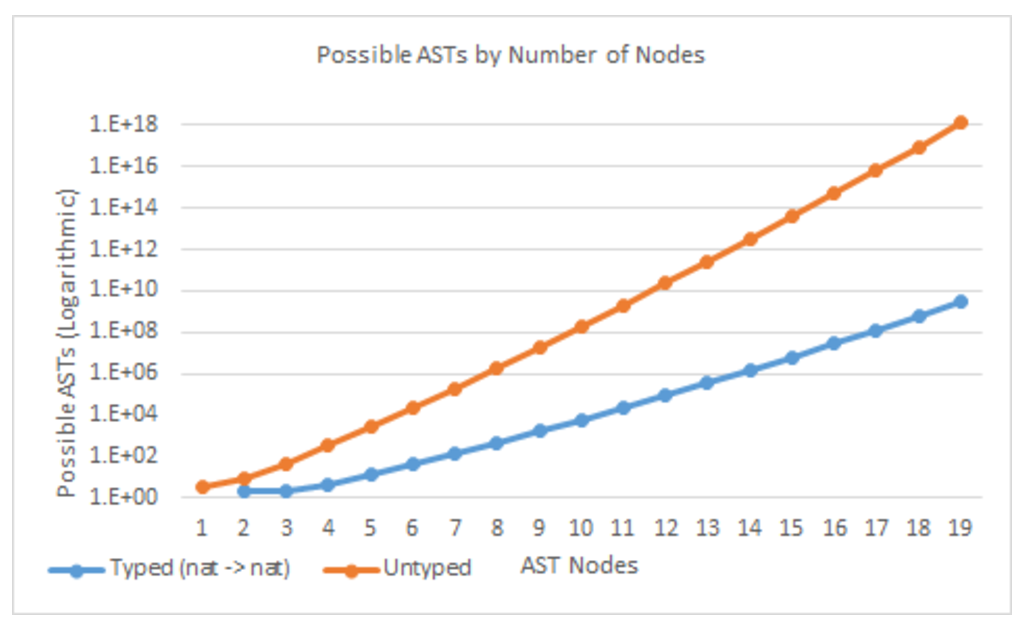
\includegraphics[width=4in]{enumeration-cropped.pdf}
\end{center}
\caption{Comparing the number of typed and untyped terms (log scale). }
\label{fig:counting}
\end{figure}

The second observation is a novel contribution of PI Zdancewic's recent work~\cite{OZ15}
and, in our view, holds
extreme promise for the construction of a new significant class of
program synthesis algorithms based on the principles of type theory.
In more detail, when checking that a function 
$\lambda x.e$ has type $\tau_1 \rightarrow \tau_2$, the standard algorithm will
hypothesize that $x$ has type $\tau_1$ and proceed with the simpler
problem of checking that expression $e$ has type $\tau_2$.  This is the
basic process by which a type checker decomposes the complex task of
checking (higher-order) functions in to the simpler task of checking
(first-order) expressions.  Analogously, when synthesizing a program
from a collection of input-output examples $\mathit{inputs}
\Rightarrow \mathit{outputs}$, an algorithm might hypothesize the
generated (possibly higher-order) program will see $\mathit{inputs}$
associated with some argument $x$.  Then, given such a hypothesis,
that algorithm might work on the simpler problem of synthesizing an
expression that produces $\mathit{outputs}$.  

A similar reduction
in complexity occurs when considering many other type constructors
as well --- not just functions.  For instance, we can type check the elements of a pair 
$(e_1, e_2)$ with type
$\tau_1 * \tau_2$ by \emph{independently} checking that $e_1$ has
type $\tau_1$ and $e_2$ has type $\tau_2$.  Likewise, we can
synthesize a program with type $\tau_1 * \tau_2$ with examples
$(\mathit{examples_1}, \mathit{examples_2})$ by \emph{independently}
synthesizing the left-hand side using $\mathit{examples_1}$ and
the right-hand side using $\mathit{examples_2}$.  Generating
$m$ possible programs for left-hand side and checking them
independently of
the $n$ possibilities for the right-hand side has a cost proportional to
$m + n$ whereas generating all pairs and checking both sides
simultaneously has a cost proportional to $m * n$.  Hence, the structural
decomposition suggested by type theory has the potential for enormous
performance gains over any naa\"{i}ve strategy.  In general, much is known about 
the structure of typed programs (often via  
the Curry-Howard isomorphism, from the structure of 
intuitionistic proofs) and it would appear that we can exploit
this structure to simplify and decompose examples
and thereby program synthesis problems.

The upshot of this new insight is that it is possible to modify the
typing rules of a programming language so that they ``push'' examples
towards the leaves of the typing derivation trees that serve as the
scaffolding for the generated program terms.  Doing so permits the
algorithm to evaluate candidate terms \textit{early} in the search
process, thereby potentially pruning the search space early.  Rather
than following the na\"{i}ve strategy of ``enumerating and
\textit{then} evaluating,'' our algorithm follows the more nuanced
approach of ``evaluating \textit{during} enumeration.''

So far, Observations 1 and 2 appear to be extremely robust both in theory and in
practice.  Indeed, in preparation for this grant proposal, we have
developed a prototype synthesis algorithm based on these two
observations~\cite{OZ15}.  
To date, the algorithm has only been designed to handle
simple recursive, algebraic data types but we have tested it on over 40
examples and found it to (a) synthesize both higher-order and
first-order programs equally well, and (b) be competitive with
existing state-of-the-art synthesis algorithms on the first-order
examples.  

Observations 3 and 4 hold great promise for the future. Because of the
correspondence between between type theory and intuitionistic logic,
we can dig in to the extensive literature on theorem proving for
intuitionistic logics~\cite{handbook-automated-reasoning} for new
kinds of algorithms that may be applied to the problem of program
synthesis.  For example, rather than search for natural deduction
proofs/programs, we can explore the use of sequent calculus-style
proofs, and we can do so either using backwards or forward search.
The literature also provides ideas for context management, program or
proof representations, and efficient data structures.  Even more
exciting, the literature on type systems has grown enormously over the
past several decades.  Types are now able to describe complex
phenomena such as strings and xml schema via regular expression types,
or complex (abstract syntax and other) trees via GADTs and refinement
types, as well as transformations between these objects.  Types are no
longer limited to descriptions of pure functions --- they can describe
computational effects as well.  Monads separate the pure from the
impure and can be used to describe simple effects such as exceptional
behavior.  Linear, affine, relevant and ordered type theories describe
the various ways in which resources may be used, providing the
possibility of rich specifications for allocating, using, updating or
consuming resources according to various protocols.  Type and effect
systems have also been used to describe memory management and to
control concurrent programs.

As mentioned above, the approach of using types and techniques from
proof search to guide program synthesis has its roots in the seminal
work by Green~\cite{green-ijcai-1969} and
Manna~\cite{manna-tse-1979,manna-plas-1980}.  What has changed in the
past forty years is three-fold: we now better understand how to
structure rich type systems and their corresponding proof theories, we
have seen how examples fruitfully enrich specifications and prune the
search space, and we now have vastly more computational resources at
our disposal.  

We are not alone in exploring applications of type theory in program
synthesis---see the work by Kuncak
\etal~\cite{kuncak-pldi-2010,gvero-pldi-2013} for one approach;
Perelman \etal{} have also used types for searching through
libraries~\cite{perelman-pldi-2012}, and Feser \etal{} have looked at
using typed combinators for synthesis~\cite{Feser:2015}.  However, to
date, there has been no systematic study of the wide variety of modern
type systems (e.g. GADTs, refinements, monadic, linear types) and how
they might be used together with examples to form the basis for an
expressive program synthesis platform.

There is also a large body of previous research on using other
techniques, such as program sketching and constraint solvers---see the
work by Solar-Lezama \etal{}
\cite{solar-lezama-thesis-2008,solar-lezama-pldi-2008,solar-lezama-pldi-2007,solar-lezama-pldi-2005}
---or computer-aided refinement of specifications---see the KIDS and
Specware
projects~\cite{smith2008generating,smith1996toward,smith1999mechanizing},
for instance.  Our type-theoretic approach is largely complementary to
these, using different algorithms, different data structures, and
different forms of specification, though we expect to incorporate
their ideas where relevant.

%Refinement: KIDS / Specware


% \dpw{We should
% mention some early type-theoretic work and cite things like swarat's work ---
% we need to defend against the reviewer who knows that there has been
% some past work on type-theoretic synthesis.} 

%To drive our research on these foundational topics and evaluate our 
%algorithms and data structures,
%we plan to study the domain of systems configuration management.
%Unix system and application configuration is often performed by
%manually editing

% \dpw{Say something about the latter two observations?  Yet another
% ``observation'' is that types are the most widely used lightweight formal
% method so they are a good means for people to specify stuff.}\saz{I
% think what you added is fine.}

%% More precisely, type theory has always been a powerful means of
%% reasoning about higher-order programs because it is compositional:
%% we can type check the elements of a pair $(e_1, e_2)$ with type
%% $\tau_1 * \tau_2$ by \emph{independently} checking that $e_1$ has
%% type $\tau_1$ and $e_2$ has type $\tau_2$.  Likewise, we can type
%% check a function (by generating hypotheses about its argument)
%% independently of any of its uses.  This compositionality allows
%% type checking to scale and programmers to work on separate modules
%% independently.  By applying similar principles to the problem of
%% program synthesis from examples, it becomes clear that if required
%% to synthesize a program with pair type $\tau_1 * \tau_2$, we can
%% instead synthesize two programs separately, one for the left-hand
%% component of the pair with type $\tau_1$, and one for the
%% right-hand component of the pair with type $\tau_2$.  Likewise, to
%% synthesis a program with function type $\tau_1 \rightarrow \tau_2$,
%% we can associate \emph{hypothetical examples} with the argument
%% $\tau_1$ and proceed to synthesize a program with type type
%% $\tau_2$.  As we decompose the structure of the program we must
%% synthesize according to its type, we also decompose the structure
%% of the examples that serve as specifications.  Eventually, given
%% arbitrary higher types and examples that match,



%% To understand why, observe first that program synthesis can, naively, 
%% be implemented as a 
%% simple-minded kind of search that enumerates one program after another
%% and as each program is generated, checks to see whether it satisfies
%% the given specification.  If you enumerate enough programs, you will eventually
%% run in to one that satisfies your specification, if such a program
%% exists.  Of course, there are many ways to enumerate programs, but Occam's Razor suggests
%% that simple programs are more likely to be the correct ones and hence an
%% enumeration that runs from the smallest to the largest programs is a reasonable
%% starting point.  

%% Of course, the enumeration can take a very long time indeed. Superficially,
%% it is clear that type systems can play a role here because
%% they dramatically cut down the number of legal programs --- a large
%% number of syntactically legal programs do not type check and can be
%% rejected immediately, without wasting time determining whether they
%% satisfy the expected examples.  Figure~\cite{fig:progs} presents a simple 
%% experiment we ran, counting the number of typed and untyped terms, presented 
%% as a log scale.  The savings for using typed terms is enormous.
%% Still, 

\paragraph*{Intellectual Merits.}
In summary, we propose a new research program on \emph{type-theoretic synthesis}
that will tackle the
problem of how to synthesize pure and effectful 
programs in their full generality.  Our proposed
research will simultaneously exploit both the structure of advanced
type systems \emph{and} the power of examples in program synthesis.
Our central research agenda will consist of four main thrusts:

\begin{itemize}
\item {\bf Core algorithms for type-theoretic synthesis.}
We will pursue fundamental research on core algorithms
and data structures necessary for type-theoretic synthesis.
Our goal is to push past current example-directed synthesis limits
by using new data structures and algorithms drawn, in part, from the
theorem proving literature.
\item {\bf Synthesis with advanced type theories.}
We will expand the expressive power of current synthesis systems by combining
specification via examples with specification in modern type theories.
In particular, we will study the use of various kinds of 
refinement and dependent types to improve the specification of pure
programs, as well as the use of monads, linear types and effects
to specify effectful computations. 
\item {\bf Theory.}
We will investigate the meta-theoretic properties of systems including
their semantics, soundness and completeness.  
%A stretch goal is to begin
%to understand what kinds of examples
%are \emph{necessary} in order to synthesize certain classes of programs.
\item {\bf Evaluation and Applications.}
Unix application and systems configuration is a messy, error-prone task:
There are countless configuration formats, all with their own idiosyncratic
formats.  We will evaluate the effectiveness of our foundational reseach 
by applying it to the concrete problem
of synthesizing custom interfaces for managing, editing, and updating these
configurations.  The programs we generate will be synthesized in the Augeas domain-specific
language for configuration management~\cite{augeas}, developed by Redhat,
and inspired by the Boomerang language~\cite{Boomerang07,bohannon2008boomerang,foster-thesis} for construction of bi-directional
programs.
% A special sub-domain of interest lies in the management of
% router configurations---such configurations are the sources of many 
% network problems
% and their management is extremely 
% challenging~\cite{feamster2005detecting,fogel+:network-config-analysis}.  PI Walker has experience in this
% domain due to his recent work on the Frenetic project~\cite{frenetic},
% which involves programming and managing networks.
\end{itemize}

%% will involve developing new data structures
%% and algorithms to improve the scaling properties of our prototype
%% and to investigate how to incorporate a broad range of more advanced
%% type theories in to our synthesis algorithms.  These new type theories
%% will include the following.

%% \begin{enumerate}
%% \item \emph{polymorphic types} to learn more general functions, 
%% \item \emph{dependent types} to further constrain functions where specification
%% via examples is inefficient, 
%% \item \emph{monadic types} to encapsulate simple effects such as exceptions, 
%% \item \emph{linear types} (to encapsulate resource utilization effects such as 
%% memory allocation), and 
%% \item \emph{advanced type-and-effect systems} to encapsulate more general
%% kinds of effect specifications.
%% In order to evaluate our ideas in practice, we propose to develop a new
%% general-purpose, higher-order, effectful and typed programming language,
%% called \OSynth{}, based around OCaml, which incorporates synthesis
%% features in to the language.
%% \end{enumerate}

\paragraph{Broader Impacts.} In the long term, there are many potential
applications of program synthesis --- it is a generally applicable
technology that can potentially benefit any area of science or
industry in which non-programming experts must write code. Combining
type-theoretic synthesis techniques with other approaches has the
potential to significantly extend the scope of program synthesis
applications.  In the short term, developing tools to synthesize new
interfaces for systems configuration will make it easier to manage
such systems and help to address 
the daunting ``UNIX configuration nightmare''~\cite{unix-config-nightmare}.
In addition, program synthesis has many
educational uses: it can be exploited to give students feedback about
programming errors, or to generate novel examples or problems for them
to work with.  

We also plan on having broad impact more directly through our educational plan.
At the undergraduate level, we plan to develop a series of undergraduate
research projects revolving around type systems, theorem proving and sythesis.
We hope that some of those projects will result in educational tools
that can be used in our undergraduate classes on functional programming.
At the graduate level, the type-theoretic approach to program synthesis 
offers a compelling pedagogical framework that touches on many modern
ideas from programming languages; that structure will be applied in
the classroom to provide course material and projects.  

The PIs have a history of engaging under-represented minorities in 
their research projects and will continue to seek out opportunities to do so.
To cite just two concrete examples, PI Zdancewic recently graduated a Filipino
student with a PhD in program synthesis, and, earlier in his career, PI Walker
mentored an African American undergraduate student who won the CRA outstanding
undergraduate award, has gone on to get his PhD in computer science, and is 
now faculty at Stanford.  Both PIs have supervised women doctoral students.

\paragraph*{Proposal Structure.}  In the following section, we further
explain our overall approach to program synthesis.  
In Section~\ref{sec:research}, we flesh out the major components of our
research agenda further.  
Section \ref{sec:impact} describes broader impacts,
Section \ref{sec:prior-support} describes our results from
prior NSF grants and Section \ref{sec:timeline} presents a
collaboration plan and research timeline.



\section{Program Synthesis with Simple Types and Examples}
\label{sec:prior}

Consider a core ML-like language featuring algebraic data types,
\cd{match}, top-level function definitions, and explicitly recursive
functions. A \emph{type-theoretic synthesis problem} is defined by: 
(1) the data type
definitions and top-level let-bindings, (2) a goal type, and (3) a
collection of examples of the goal type.  The synthesis task is to
find a program of the goal type that is consistent with the examples.
Figure~\ref{fig:stutter} presents a simple example of such a synthesis 
problem, as well as an expected result.
To obtain such a result, our type-directed synthesis algorithm
performs two major operations: \emph{refining}
the constraints, the goal type and examples, and \emph{guessing} a
term of the goal type that is consistent with the example values.

\paragraph{Term guessing by enumeration.}
Guessing amounts to systematic enumeration of candidate terms in
increasing size, followed by evaluation in context to see whether they
agree with the current set of goal examples.  Because we are operating
in a statically-typed setting, we avoid enumerating ill-typed terms,
which rules out nonsensical expressions like \cd{Nil Cons} (of which
there are exponentially many for a fixed term size).  However, there are
still many well-typed terms that we also wish to avoid. For example, a term
that matches against a constant constructor, like \cd{match Nil with
  Nil -> e1 | Const -> e2} is equivalent to a smaller term that has no
\cd{match} (in this case \cd{e1}).  And to make matters worse, there
are an infinite number of these bad terms, obtainable by introducing
additional lambdas and applications.  To avoid these sorts of
redundant terms, guessing only generates $\beta$-\emph{normal forms}:
terms that can be reduced no further.



\paragraph{Refinement.} The process of using type and example
constraints to guide the search process is refinement.  As an example,
consider searching for solutions to the \cd{stutter} example of
Figure~\ref{fig:stutter}.  Already from the goal type \cd{list ->
  list}, we know\footnote{To rule out generation of many redundant expressions, we
generate terms in \emph{eta-long} beta-normal form,
which mandates that terms of type $\tau_1 \rightarrow \tau_2$ be
function definitions as opposed to other expressions that compute
functions.}  that the top-level structure must be of the form 
below.

\begin{center}
\cd{let rec f1 (l1:list) : list = ? }
\end{center}

\noindent  When synthesizing the body of
the function, the examples tell us that in the ``world'' (\ie\ a
hypothetical evaluation of \cd{stutter}) where \cd{l1} is \cd{[]} the
expected answer is \cd{[]} and, in similarly in the world where
\cd{l1} is \cd{[0]} the expected answer is \cd{[0;0]}.  So each such
input--output pair becomes a new example ``world'' where the output
value is the goal and \cd{l1} is bound to the corresponding input
value.

To fill in the body of the function, which must be a term of type
\cd{list}, we observe that no single list constructor agrees with the
examples (since there are examples starting with both \cd{Nil} and
\cd{Cons}).  Hence guessing either \cd{Nil} or
\cd{Cons} is contradicted by examples.
We also try guessing terms that involve variables:
the smallest well-typed such term in this context is \cd{l1}, but that also
does not agree with the examples.  The larger terms all involve
\cd{stutter l1}, which is well-typed, but not structurally recursive, so it
is also discarded.

With these possibilities exhausted, we next consider introducing a
\cd{match} expression.  We first guess possible scrutinees to
\cd{match} against: they must have algebraic types and be terms
constructed from variables in the context.  The only such term in this
case is \cd{l1}, so we consider refining the body of the function to:

\begin{figure}[t]

\begin{minipage}[t]{3.5in}
{\small
\begin{lstlisting}
(* Type signature for natural numbers and lists *)
type nat =              type list = 
  | O                      | Nil
  | S of nat               | Cons of nat * list
(* Goal type refined by input/output examples *)
let stutter : list -> list |>
  { []      => []
  | [0]     => [0;0]
  | [1;0] => [1;1;0;0]
  } = ?
\end{lstlisting}
}
\end{minipage}
\quad
\begin{minipage}[t]{3in}
{\small
\begin{lstlisting}
(* Output: 
 * synthesized implementation of stutter *)
let stutter : list -> list =
let rec f1 (l1:list) : list =
  match l1 with
   | Nil -> l1
   | Cons(n1, l2) -> 
      Cons(n1, Cons(n1, f1 l2))
in f1
\end{lstlisting}
}
\end{minipage}
\caption{An example program synthesis problem and the resulting
  synthesized implementation.  }
\label{fig:stutter}
\vspace{-3ex}
\end{figure}


\begin{center}
\cd{match l1 with Nil -> ? | Cons(n1,  l2) -> ?}
\end{center}
\noindent When pattern matching, we distribute the evidence
according to how the \cd{match} evaluates in each example world.
In this case, \cd{l1} evaluates to \cd{Nil} in the first world and
\cd{Cons(_,_)} in the other two worlds.  Therefore, we
send the first example to the \cd{Nil} branch and other
two examples to the \cd{Cons} branch.  We are left with two
sub-goals in refined worlds.  The \cd{Nil} case follows immediately:
the only example left in the goal is \cd{Nil} and there are two ways
to generate it: the constant \cd{Nil} constructor or \cd{l1}.

\paragraph{Recursive Functions.}
The \cd{Cons} case proceeds with another round of guessing, but the
solution requires a recursive call to \cd{f1}.  How might we generate
a recursive function in this type-directed, example-based style?  The
answer is that when introducing a recursive function like \cd{f1}, the
input-output examples for the function itself, interpreted as a
partial function, serve as a reasonable approximation of its behavior.
Here, the example for \cd{f1} in all three worlds would be the partial
function given by all three examples.  Given this information in the
context, the guessing procedure can quickly determine that 
\cd{Cons(n1, Cons(n1, f1 l2))} is a solution for the \cd{Cons} branch
of the match. 

\paragraph{Formal System.}
The algorithm we have just described informally can be described formally
via a collection 3 mutually recursive judgements:

\begin{itemize}
\item $\Gamma \vdash \tau \ \& \ e \leadsto I$:
A judgement directed by the syntax of a goal type $\tau$ and a
collection of examples $e$, to synthesize
an introduction form $I$, such as a function, a pair or a constructor.
\item $\Gamma \vdash \tau \leadsto I$: A judgement to guess an introduction 
form of type $\tau$ by enumerating all possible well-typed introduction forms.
\item $\Gamma \vdash \tau \leadsto E$:  A judgement to guess an elimination 
form (ie: a variable $x$ from the context, or a function application or
a projection) by enumerating all possible elimination forms of a type.
\end{itemize}
 
\paragraph{Results so far.}  Figure~\ref{fig:maindata} presents a
selection of the synthesis results we have obtained so far, focusing
on the case for simple lists.  For each entry of the table we verified
by manual inspection that the resulting synthesized program was a
correct implementation of the desired outcome.  Synthesis time appears
competitive with other approaches, the most closely related of which
is the Escher system, by Albarghouthi~\etal~\cite{albarghouthi-cav-2013}.  Yet, unlike those
other approaches, we are able to synthesize functions with
higher-order types such as map and fold just as easily as first-order
types.

\newcommand{\maindataCount}{ 43 }
\begin{figure}[t]
  \begin{center}
  \tabcolsep 5.8pt
  \footnotesize
  \begin{tabular}{|c|c|c|c|c|}
  \hline
  \textbf{Test} & \textbf{ \#Ex } &
  \textbf{ \#N } & \textbf{T (Ctx)} & \textbf{T (Min)} \\
  \hline

%%%%% TABLE DATA
list\_append & 12 & 12 & 0.011 & 0.003 \\
\hline
list\_compress & 13 & 28 & 128.339 & 0.073 \\
\hline
list\_concat & 6 & 11 & 0.019 & 0.006 \\
\hline
list\_drop & 13 & 13 & 1.29 & 0.013 \\
\hline
list\_even\_parity & 7 & 13 & 0.518 & 0.004 \\
\hline
list\_filter & 8 & 15 & 1.327 & 0.013 \\
\hline
list\_fold & 9 & 13 & 0.504 & 0.139 \\
%\hline
%list\_hd & 3 & 5 & 0.019 & 0.001 \\
\hline
list\_inc & 4 & 8 & 0.004 & 0.00 \\
%\hline
%list\_last & 6 & 11 & 0.093 & 0.00 \\
\hline
list\_length & 3 & 8 & 0.019 & 0.001 \\
\hline
list\_map & 8 & 12 & 0.082 & 0.008 \\
\hline
list\_sort\_sorted\_insert & 7 & 11 & 0.009 & 0.008 \\
\hline
list\_sorted\_insert & 12 & 24 & 22.016 & 0.122 \\
\hline
list\_stutter & 3 & 11 & 0.018 & 0.001 \\
\hline
list\_sum & 3 & 8 & 0.005 & 0.002 \\
\hline
list\_take & 12 & 15 & 1.147 & 0.112 \\
%\hline
%list\_tl & 3 & 5 & 0.02 & 0.001 \\

  \hline
  \end{tabular}
  \end{center}
  \caption{Aggregated benchmark suite results. For each test, we report the number of given examples (\#Ex), the size
  of the result (\#N), and times taken in seconds to synthesize in a populated context (Ctx) and minimal context (Min).}
  \label{fig:maindata}
  \vspace*{-2.5ex}
\end{figure}


\section{Research Agenda}
\label{sec:research}

In this section, we discuss our core research proposal.

\subsection{Core Algorithms for Type-theoretic Synthesis}
\label{sec:core}

Fundamentally, efficient program synthesis requires algorithms
that can search the space of possible programs rapidly.
Our prototype system incorporates several key ideas that
help cut down this search space:  We use \emph{examples} in addition
to types throughout the synthesis process; 
we search only for \emph{eta-long}, \emph{beta-normal} forms; 
we build efficient data structures called
\emph{refinement trees} to avoid enumerating 
the same programs more than once; and we carefully manage the type-checking
context.  Still, we plan to research a number of additional ways to 
improve the search process.

\paragraph*{Beyond eta-long, beta-normal Form.}
By enumerating only the functions in eta-long, beta-normal form, we avoid 
constructing or testing many programs.  A key question is how
to cut down the search space even further --- there are still many programs
in eta-long, beta-normal form that are semantically equivalent.
One possibility is to bring stronger equational theories, such as the theory
of rings, groups, lists or arithmetic, in to the search process.  For example,
we plan to investigate variations of our search process that incorporates
congruence closure algorithms~\cite{shostak:congruence,nelson-oppen,sjoberg:congruence} for
computing term equivalence.  We hope to find a way to
sample just one representative from each equivalence class of terms
rather than many.  However, we anticipate there will be a trade-off
between the cost of computing closures and the benefits gained from using
them.  More research is required to determine the nature of this tradeoff.

\paragraph*{Search order variations.}
Our prototype synthesis algorithms are inspired by top-down natural
deduction proof strategies.  However, as the range of type constructors
we consider expand, there are some search-order variations we can consider.
For instance, even adding ordinary tuples (pair types) introduces a new
set of interesting choices:  tuple components can be extracted once and
eagerly, as soon as possible, or lazily on demand.  It is unclear which 
will perform better.  When it comes to more sophisticated type constructors,
especially polymorphic types, further choices will likely reveal 
themselves (see also the discussion of polymorphism in 
Section \ref{sec:types} below).
In addition, entirely different search-orders that combine some bottom-up proof search in addition to our general top-down approach may perform well
in certain circumstances.  We plan to evaluate such possibilities.

\paragraph*{Reducing example requirements.}
One of the weaknesses of our current approach is that when our recursive
divide-and-conquer algorithm considers how to synthesize different
branches of a match statement, it does so independently.  This is 
both a blessing and a curse: independence limits the combinatorial
explosion, but it also means that we can't reuse the parts of a function
that we have already synthesized.  As a consequence, we sometimes need 
extra examples, particularly when synthesizing recursive functions.
We plan to develop new techniques (which we call \emph{recursive back-patching
algorithms}) that will allow us to use portions of a function we have
already synthesized instead of requiring additional examples.

\paragraph*{Incorporating negative examples.}
Our algorithms so far use \emph{positive examples}. For instance,
the example \texttt{\{0 => 1\}} states the function we desire transforms
\texttt{0} in to \texttt{1}.  However, users can also give \emph{negative
examples} that state undesirable behavior.  For instance, Le and Gulwani~\cite{vu-pldi-2014} developed a user interface for data extraction
that allows users to select ``good'' (positive) examples of text
they would like to extract from a file and as well as ``bad'' (negative)
examples of text they do not want to select.  The combination of good
and bad information helps refine the extraction algorithm.  More generally,
there are some classes of functions, such as regular expressions,
which can be learned with both positive and negative examples
but cannot be learned with only positive examples~\cite{gold:inference}.  
We will
investigate how to incorporate negative examples in to our
work.  Whereas our current algorithms are linked, via the Curry-Howard
isomorphism, to proof search
in constructive logics, we may find a link to classical logics when
we begin to study the consequences of having negative examples.
More specifically, we will investigate the notion of an example
of a \emph{contradiction} (the key judgemental notion that 
arises~\cite{pfenning:classical}) 
in an attempt to get to the heart of how learning
from examples interacts with classical logic.

\paragraph*{Data structure optimization.}
Our current prototype includes little work optimizing the basic data
structures or the evaluator we use.  Throughout the
course of the grant, we will look for ways to optimize the core enumeration
and evaluation algorithms.

\subsection{Beyond Simple Type Systems}
\label{sec:types}

Our prototype currently operates over simple, recursive algebraic
data types.  We intend to enrich the type theory of our synthesis
system in several different directions.

\paragraph*{Polymorphic Types.}

The first natural major extension to our system is to add
parametric polymorphism, which will allow us to synthesize generic
functions.  Some of the standard OCaml collection libraries, such as
the List module, will serve as good benchmarks to evaluate our success
here.  There will be several challenges involved in synthesizing 
polymorphic programs.  First, since our core algorithms are directed by
the desired type of our resulting expression, when we synthesize 
that expression, we may need to search for polymorphic functions, which
when instantiated with particular type arguments, can generate results 
of the expected type.  
We anticipate incorporating unification of goal types in to our search
process to achieve such results.  Second, thanks to Reynolds' parametricy
theorem~\cite{reynolds:parametricity} and Wadler's work on ``theorems for free''~\cite{wadler:theorems-for-free}, it is well known that there are simply
``not very many'' functions of certain polymorphic types.  For instance,
the only functions with type $\forall \alpha. \alpha \rightarrow \alpha$
are the identity function and the function that does not terminate on
any input.  When searching for polymorphic functions, we should be able
to exploit this fact to dramatically cut down the search space, especially 
if we are given effective examples.  On the latter point, 
Voigtl\"{a}nder~\cite{voigtlander:bidirectionalization-for-free}
shows how to construct examples in a particular way, and then to exploit 
parametricity to infer
the inverse of a given function.  We will examine his methods to determine
whether similar concepts can be used in a more general synthesis setting.
Finally, we are interested in examining whether we can use polymorphism
to help us vary the synthesis search order in effective ways.
For instance, even if the type of program we are looking for, say 
$\mathit{int} \rightarrow \mathit{int}$, is not polymorphic, we might
begin the search by looking for an abstraction of that function, perhaps
$\alpha \rightarrow \alpha$, for which (by parametricity) there are fewer
exemplars.  If that fails, we might look for the more concrete
functions $\mathit{int} \rightarrow \mathit{int}$.  Alternately,
when looking for a function with type $\mathit{int} \rightarrow \mathit{int}$,
we might actively \emph{avoid} looking for functions that can also have type
$\forall\alpha.\alpha \rightarrow \alpha$ under the assumption that if the 
user wanted
a polymorphic function, they would have supplied a more general type.
Either way, we hope that polymorphic typing can be used in new ways
to help guide the search for programs that satisfy a specification.

\paragraph*{Generalized Algebraic Datatypes}

A second natural extension, once polymorphic types are available, is
to include generalized algebraic datatypes (GADTs), which can be
thought of as extending ordinary polymorphic datatypes with extra
equality constraints.~\cite{middelkoop2010lean} Such equality
constraints allow more invariants to be expressed within the type
language---for instance, it is possible to encode invariants about
various kinds of balanced-tree structures.  
We anticipate that GADTs
will fit naturally in to our type- and example-directed synthesis
approach because they enjoy a tractable type inference
algorithm~\cite{schrijvers2009complete}. The additional equality
constraints imposed by GADTs should provide information that can help
prune the search space, though determining the most fruitful way to
take advantage of the extra equalities is one clear direction for
research. 

\paragraph*{Refinement Types.}
In 1991, Freeman and Pfenning introduced a notion of \emph{refinement type}
to Standard ML~\cite{freeman:refinement-types}.  Refinement types extend
the ML type system with the ability to specify specializations of data
types.  For instance, the standard list type definition:
\begin{verbatim}
datatype 'a list = nil | cons of 'a * 'a list
\end{verbatim}
can be refined by a refinement specification:
\begin{verbatim}
reftype 'a single = cons ('a, nil)
\end{verbatim}
The refinement defines a new subtype of lists that is inhabited
by lists with exactly one element.  In Freeman's work,
programmers can use such refinement
types in conjunction with intersection and union types to provide
much richer specifications of programs than are possible in 
the Standard ML type system.  Since, Freeman's initial work,
many others have experimented
with effective variations and extensions~\cite{pfenning:refine-logic-frameworks,davies:refinement-checker,davies:refine-checking,vazou:abstract-refinements}

We believe that refinements, together with intersection types,
may provide an effective framework for more deeply understanding
synthesis from examples and for generalizing all of our existing
algorithms.  More specifically, we have made the observation 
that one of our existing 
example function specifications (shown on the left)  can be
reinterpreted the refinement type (shown on the right)!

\noindent
{\small
\begin{lstlisting}
  { []    => []                                            []    -> []        /\
  | [0]   => [0;0]                                         [0]   -> [0;0]     /\
  | [1;0] => [1;1;0;0] }                                   [1;0] -> [1;1;0;0] 
\end{lstlisting}
}
\noindent
We believe this surprising and exciting observation will open the door
to reinterpreting program synthesis with types and examples as pure
type-theoretic synthesis procedure (without examples).  One of the main
advantages of this new viewpoint is that we hope to be able to exploit
even more of the theorem-proving literature as the link between intersection
types and conjunction should be relatively 
clear whereas the sets of examples that we had been using had no obvious
theorem-proving analogue.  

In addition, this insight suggests new kinds
of ``examples'' that we hope to be able to incorporate in to our system.
For instance, the refinement of lists first suggested, \verb+cons ('a, nil)+, 
may be interpreted as a \emph{symbolic example}, with some parts of the
example concrete and other parts abstract.  It specifies that a list 
must have one element, but allows that element to be anything at all.
A symbolic example of the form:

\noindent
{\small
\begin{lstlisting}
  { cons ('a, nil) => cons ('a, cons ('a, nil)) }
\end{lstlisting}
}

\noindent
provides more information than the analogous concrete specification:

\noindent
{\small
\begin{lstlisting}
  { cons (0, nil) => cons (0, cons (0, nil)) }
\end{lstlisting}
}

\noindent
In the first case, we are effectively specifying an infinite family of
examples (a function) all at once.
We are eager to experiment with program specifications involving such
symbolic examples and to implement synthesis procedures for them.
We believe that in many cases,
such specifications may provide programmers with
betters ways to express their intentions than with examples alone.
In general, symbolic examples, intersection types and refinement
types provide a much more general specification mechanism than
simple types and examples provide separately.


\paragraph*{Dependent types and integration with SAT and SMT.}
Freeman and Pfenning's refinement types make it possible to
specify more properties of a program in that program's type signature
than is possible in a simply-typed or polymorphically typed program.
However, they do not allow specifications to use the rich
theories, such as those for uninterpreted functions, arithmetic, sets
and arrays, available in modern SAT and SMT solvers such as Z3~\cite{Z3}.
We also plan to investigate extensions that include
dependent types $\Pi x{:}\tau_1.\tau_2$ and constraints $\{x{:}\tau \, | \, P(x)\}$.
Such types will provide mechanisms for more precise specifications
than would otherwise be possible with refinements alone.  In order
to solve synthesis problems in the contexts of such constraints,
we anticipate having to combine our type-theoretic approaches with the
SAT- and SMT-based synthesis approaches used in other 
work~\cite{alur-fmcad-2013,solar-lezama-thesis-2008,vu-pldi-2014}. 
A particularly compelling use for such richer, potentially dependent
types, is to augment the language with primitives for strings and
regular-expression refinement types.  Such types have found use in the
context of semi-structured (e.g. XML or HTML) data
transformation~\cite{hosoya2003xduce,benzaken2003cduce}  and in the work on
bi-directional programs, or \textit{lenses}~\cite{foster2007combinators,bohannon2008boomerang},
that provide succinct ways of reconciling differing views with updates
of data.  Relatively recent work~\cite{henglein2011regular} has shown how to give a computational interpretation to
regular expression types more generally.  Here, the richer type
structure should suggest domain-specific synthesis strategies that we
intend to apply in the context of data transformation
applications---see Section~\ref{sec:appl} for a description of one use case for 
  configuration files.

% - used in xduce, cduce, lens languages 
% - for working with strings and semi-structured data like XML 
% - synthesize program transformations 
% - Henglein
% - [forward reference to example applications]


\paragraph*{Effectful programs.}

The various ways of enriching type systems described above pertain
mainly to the synthesis of \textit{pure} programs.  However, many
applications of  program synthesis are best framed in languages that
support \textit{effects}, which allow for features like exceptions,
resource management, concurrency, or other kinds of I/O.   We will
therefore investigate ways to extend our type-directed synthesis
techniques so that they apply in these settings as well.

The programming languages research community has identified several
type-theoretic approaches for expressing effectful computations, and
they should be conducive to our type-directed synthesis approach.  One
simple example is a type system that tracks exceptions~\cite{leroy2000type}.  In this case, the presence of an exception
in a function' signature constrains its implementation so that either
it relies another function that raises a (compatible) exception or it
raises the exception itself.  Dually, the lack of an exception in the
function's signature indicates either the function has a local
exception handler or it does not rely on other exception-producing
functions.  In any case, these types constrain the search space of
possible implementations.  A related approach is to use
\textit{monads}~\cite{moggi1991notions,wadler1998marriage}, which are well known to be able
to describe effectful computations and also have a close correspondence
with the type-and-proof-theoretic search strategies that we employ.
In particular, the notion of $\beta$-normal
$\eta$-long programs can be naturally extended to include monadic
canonical terms that define where effects may occur~\cite{concurrent-logical-framework-propositional,watkins2003concurrent}.  How best to utilize such insights in program synthesis is an important
question we intend to investigate.

Another promising avenue is to explore program synthesis in the
context of \textit{linear types}~\cite{Girard87}, and the related notion
of \textit{session types}~\cite{CairesP10concur,VasconcelosGR06multithreaded,wadler2014propositions}.  These techniques
permit the program's type system to capture properties of resource
usage or communication patterns.  For instance, recent work by
Pfenning and Wadler has shown how linear types give rise to session
types that can encode protocols.  Here, the strong connection to logic
and proof theory suggest that our type-directed synthesis techniques
could be used to find implementations of protocols.

One challenge in the synthesis of effectful programs is how to extend
the ``input/output'' examples: I/O examples alone are not
sufficient in the presence of effects---we also need specifications of
the intended side effects.  One possibility is to define classes of
behaviors, possibly by combining monadic or linear type systems with
richer SMT-based constraints.


\subsection{Theory}

Our research philosophy demands that we make progress on theoretical
analysis of our programming languages and tools at the same time as
we implement them:  theory informs practice and practical experiments
suggest new theoretical avenues to pursue.  We will adhere to this
philosophy as this project evolves.

\paragraph*{Semantics of Underdefined Programs.}
Our current prototype involves extending OCaml with ``holes'' that
can be filled with synthesized programs.  The first natural question
that arises is how to give a semantics to such a language.  Our
initial investigations in to this topic have lead us to the work of
Denney~\cite{denney:underdeterminism}, who developed a semantics for a simply-typed
lambda calculus with ``underdefined'' subprograms.  Denney was interested
in studying the semantics of manual program refinement from specifications 
as opposed to program synthesis.  Nevertheless, his basic theory may be 
applicable, though he does not consider polymorphism, recursion, sum
types or dependent types.  We plan to explore extensions of this theory 
to provide a semantics and equational theory for our language.

\paragraph*{Soundness and Completeness.}
Two key meta-theoretic properties of our synthesis systems are
\emph{soundness} and \emph{completeness}.  In order for our system
to be \emph{sound}, any program we synthesize must be well-typed
and consistent with our examples.  We have discovered that in the
presence of recursive functions, the soundness of our divide-and-conquer
algorithms is somewhat subtle.  More specifically, when synthesizing
a sub-part of a recursive function $f$, it is tempting to use a recursive
call $f e$ in certain circumstances.  However, we have discovered that in
the context of our current algorithms, it is
only sound to do so if the correctness of the call $f e$ can be validated
\emph{locally} by an example.  However, this leads us to require more examples
than expected.  We plan to investigate this issue more deeply, both in
theory and in practice --- it is closely connected to the 
\emph{recursive back-patching} procedure (see Section~\ref{sec:core}), 
which uses more global
information during synthesis.  

A well-specified form of \textit{completeness} for our algorithms
is also clearly also an important goal:  Completeness is one of the principles
that separates ad hoc, heuristic techniques, whose effectiveness is hard to 
understand, from principled techniques whose limits are better understood.
%In general, a complete procedure is one that, given enough time,
%is guaranteed to generate a well-typed program consistent with the examples
%given if one exists.  
One of the major challenges in defining (and achieving)
completeness in our setting is that we are synthesizing \emph{higher-order}
programs that may involve the use of \emph{higher-order} examples -- in
other words examples that involve functions as arguments or results of
other functions.  When we synthesize a program, we must check that it is 
consistent with the examples provided and doing so devolves to checking
equivalence of functions.  At the moment, our system is conservative,
and uses an intentional, syntactic definition of function equivalence.
An initial goal is to prove completeness with respect to this simple
definition of function equivalence.  A more challenging goal involves
considering more liberal notions of function equivalence and attempting
to understand how such notions might suggest changes or otherwise
inform us about the properties of the algorithms we use.

\subsection{Applications and Evaluation:  Systems Configuration Management}
\label{sec:appl}

In order to evaluate our algorithms, we will measure their
effectiveness on both micro-benchmarks and larger 
applications.  
One application domain that we propose to study in detail is the domain
of systems configuration and configuration management.
At the moment, many Unix-style systems and applications are managed 
by manually editing collections of cryptic configuration files.  
To parrot Matthew Arnison's article on
\emph{How to fix the Unix configuration nightmare}~\cite{unix-config-nightmare}---this is a mess.  These configuration files
come in a host of different ASCII formats, and correctly finding,
editing, and maintaining entries is a challenge.  

Recently, however, RedHat has developed Augeas~\cite{augeas}, a new, typed,
\emph{bi-directional} language, based on Boomerang~\cite{Boomerang07,bohannon2008boomerang,foster-thesis}, 
to help support configuration file
management.  We call Augeas a bi-directional language because every
Augeas program constructs two functions at once:  one function that maps
a configuration file to a higher-level \emph{view}, and a second
function that maps the higher-level view back to a configuration file.
We typically call the function from file to view the \emph{get} function
and the function view to file the \emph{put} function.  Together,
the pair of functions is a \emph{lens}.
The semantics of Augeas (and Boomerang) guarantees that 
\emph{get} and \emph{put} functions satisfy a number of 
algebraic laws,
making them proper ``inverses'' of one another.

%As an example, consider the process of converting a configuration
%file containing a string with a key and a value:\footnote{This example
%drawn from the Augeas tutorial~\cite{augeas-tutorial}.}
%\begin{verbatim}
%key = value
%\end{verbatim}

Overall, Augeas programs support configuration management
by providing users with simpler, higher-level, and
more uniform interfaces for managing configuration files.  
Moreover, while the user manipulates the high-level interface,
the legacy system can query the low-level configuration file.
The bi-directional program keeps the view and the low-level configuration 
correctly in sync by mapping data back and forth.
However, despite its elegant design, Augeas still has a significant learning curve.
For instance, while Augeas has been integrated in to the IT management
system Puppet~\cite{puppet},
the maintainers complain that ``many lenses are not documented sufficiently, or at all'' and that figuring out how Augeas maps files into
views is ``unfortunately complicated~\cite{augeas-complicated}.''

We believe that Augeas together with program synthesis may be 
able to further ameliorate the configuration file management problem.
In particular, we plan to exploit the fact that Augeas is \emph{typed}
(meaning our type-directed algorithms apply), Augeas schemas and
update commands are often relatively \emph{short} (meaning synthesis has a
chance to be tractable in this domain), and Augeas (and Boomerang)
have \emph{bindings in OCaml}, meaning the mechanics of interfacing
Augeas with our existing OCaml infrastructure should be seemless.
There are two synthesis scenarios that we intend to investigate, which
we detail below.

\paragraph*{Synthesis of common configuration transformations.}
Augeas already has a library of programs for presenting views of 
common configuration files.  These programs convert the configurations
into trees, which may then be manipulated by user commands to query and
update the trees.  The sequence of user commands can be quite short 
(and hence effective synthesis targets) but they are
still relatively cryptic.  As a simple example, to add a new element to
the \verb+/etc/hosts+ file (which already has an Augeas schema in the
standard library), one writes the following in Augeas:
\begin{verbatim}
set /files/etc/hosts/01/ipaddr 192.168.0.1
set /files/etc/hosts/01/canonical pigiron.example.com
set /files/etc/hosts/01/alias[1] pigiron
set /files/etc/hosts/01/alias[2] piggy
save
\end{verbatim}
Of course, if adding hosts in this way is a common task, 
one might prefer to wrap the boilerplate in a script and 
use a much lighter weight interface such as the following:
\begin{verbatim}
add_host 192.168.0.1 pigiron.example.com [pigiron; piggy]
\end{verbatim}
With more engineering, one could also potentially generate a user-friendly
GUI.
We propose to use the information in the Augeas lens for  \verb+/etc/hosts+,
which contains both information on the format of the hosts file as well as 
types describing the shape of the resulting tree, together with
examples to drive the synthesis of such scripts.  By synthesizing
reuseable scripts from configuration change logs stored in a git repository,
we believe we will be able to provide users with new custom interfaces
that will faciliate execution of their most common tasks.

Notice that the scripts have
effects --- they update fields and save results --- and have a monadic
structure.  Moreover, 
operations in the script are constrained by the type of tree being 
transformed and such tree types are constrained by regular expressions,
which control the format of the field.  All in all, this combination---recursive tree types, effects, monads, regular expressions---poses
a number of interesting challenges for type- and example-directed synthesis.  
Our foundational work will be well-tested by this application domain.


\paragraph*{Synthesis of new Augeas programs.}  
While Augeas comes with a library of lens programs, it is far from
complete and never will be---there are always new applications 
and new configuration files.
Hence, a second goal is to synthesize new Augeas lenses that map
relevant portions of new configuration files into high-level views.
The inputs to this problem will include:  (1) example configuration
files, (2) types describing the shape of the view, and (3) example
view elements.  
Notice how this problem differs from the problem studied by
Srivastava \emph{et al.}~\cite{srivastava-pldi-2011}.  Srivastava
shows that given an imperative program, such as a compression algorithm,
one can synthesize the program's inverse (a decompression algorithm).  We plan to synthesize
both the program and its inverse at the same time; the algorithms
we need to do this are entirely different.

A significant additional challenge in this domain will arise from
the need to learn the grammar of the underlying configuration
file---a significant portion of any Augeas computation involves
parsing regular grammars.  Fortunately, PI Walker has studied related problems
extensively in the past in the context of the PADS project~\cite{fisher+:pads,fisher+:popl06,fisher+:jacm}.
In that work, PI Walker and his collaborators showed how to
synthesize the formats of system logs, such as apache log files~\cite{fisher-popl-2008,qian:markup}.
We conjecture a number of the algorithms used there,
which were based on recursive divide-and-conquer style
synthesis and used information-theoretic metrics to guide the search, 
will be applicable in this context as well.  In addition, we will exploit
insights from Gulwani and others on data extraction and
synthesis of string transformations~\cite{itzhaky-oopsla-2010,harris-pldi-2011,gulwani-ppdp-2010,vu-pldi-2014}.



%% \paragraph*{Target Sub-domain: Router Configurations.}
%% One subdomain of particular interest involves management of 
%% router configurations.  Router configurations are notoriously 
%% difficult to configure and maintain properly.  A series of projects
%% over the years in the networking community has attempted to catalogue
%% common errors and to define analyses to detect 
%% them~\cite{feamster2005detecting,fogel+:network-config-analysis}.
%% In particular, \emph{provisioning}, the process of deploying new
%% equipment in a network, can be quite error prone as it may  
%% necessitates making changes to
%% a number of different device configurations. 

%% At Princeton, Hyojoon Kim was recently hired to
%% manage experimental new OpenFlow networks being deployed at Princeton.
%% Joon, a former PhD student of Nick Feamster, Princeton Networking Professor, has
%% access to a github repository that records changes to network configuration
%% files.  This repository will
%% allow us to study the details of real-world network configuration.
%% In addition, we will extract examples of configuration changes from the git
%% logs to feed to our synthesis engine.  We will
%% use it to experiment with the process of learning useful new configuration
%% transformations.


%\paragraph*{Related Work.} \dpw{Do we need this subsection here?  Right now
%this is just a placeholder to remind us to say something somewhere.} 




%% The natural way to evaluate the synthesis algorithms that we devise is
%% to implement them and experimentally determine their effectiveness on
%% various synthesis tasks.

%% We have already begun to build a prototype implementation of a
%% programming language that supports the example-driven type-directed
%% synthesis proposed here.  The prototype accepts a (monomorphic) subset
%% of the OCaml programming language, extended with a simple form of
%% ``holes'' and syntax for input--output examples.  The code in
%% Figure~\ref{fig:stutter} shows a valid input to our tool.  We intend
%% to extend the tool's implementation in tandem with the theoretical
%% developments of this research.

%% In the course of building our initial prototype, we assembled a suite
%% of over 40 different programs and corresponding suites of examples to
%% attempt to analyze.  Most of these programs process booleans, lists
%% and trees.  A few are more ambitious.  For instance, we have attempted,
%% but failed so far, to synthesize a type checker for the simply-typed
%% lambda calculus---being able to synthesize that program, which
%% requires non-trivial nested conditional reasoning, will be a good test
%% of our progress.   There are many other programs that are out of reach
%% of our current synthesis capabilities, and we expect that the ideas
%% proposed here will significantly extend the reach of our algorithms.

%% There are several important metrics that we will measure as part of
%% our experimentation: the required number of examples, the synthesis
%% time and memory required to synthesize the given programs, as well as
%% the relationship between synthesis time and the size of the ambient
%% context.

%% As we increase the number of features supported by our system, we
%% will be able to extend the scope of our examples.  One major goal 
%% of the project is to be able to synthesize the complete, pure, subset of several
%% of the OCaml libraries.  In particular, once we have developed techniques
%% for inferring polymorphic programs, we will target the OCaml list
%% library (\url{http://caml.inria.fr/pub/docs/manual-ocaml/libref/List.html}).
%% The success of this proposal may be evaluated in part based on our
%% ability to synthesize the contents of such libraries.

\section{Broader Impacts of the Proposed Work}
\label{sec:impact}

In the long run, there are many potential broader impacts for our
proposed research.  We have chosen to focus on one particular application
area, systems configuration management, because having a concrete objective
and set of benchmarks is an effective means of driving the research forward,
and also because we believe that improvements in systems configuration
can lead to more reliable, easier to maintain systems that will have
a broad impact on society.
Neverthless, as discussed in the introduction, program
synthesis is a generally applicable technology, and, as such, it can
potentially impact many diverse areas of science and industry.
In addition, because it makes programming tasks more accessible, any scenario in
which non-programming experts spend significant time coding can
potentially benefit from synthesis.  

%% This project aims to study foundational techniques for synthesizing
%% programs.  In practice, it is likely that a combination
%% of approaches, leveraging the strengths of each, would be used.  SMT-
%% and SAT-solver based techniques work well in some domains, while our
%% techniques apply mainly to tree-structured data.  Our
%% example-driven approach is closely related to program testing, which
%% is already extremely widely used in industry.  In the long term,
%% program synthesis techniques could therefore (partially) automate
%% test-driven development.  It is also likely that example-driven
%% synthesis will interace well with other forms of testing and/or
%% program verification. \dpw{should the above paragraph be cut?}

In the short term, one exciting potential application of synthesis
technology is to improve education tools for computer science
courses~\cite{singh-pldi-2013}.  One use case would be to exploit
synthesis to give students automated feedback about their programs:
given a partially completed program, one could imagine a tool that
uses synthesis to interactively give hints or suggestions about how
the student should proceed.  Another possibility would be to have a
tool that demonstrates how higher-order functions such as \cd{map} and
\cd{fold} can be used: given a student's program implemented without
using \cd{map}/\cd{fold}, the synthesizer could find (if possible) an
equivalent implementation that uses them.  Such synthesis tools could
also potentially be used to automatically generate many variants of
simple programming exercises, which could be used to help students
practice their programming skills.  These synthesis tasks are almost
already within the scope of what our prototype implementation can
already handle, so we are optimistic about the possibility of
employing them.  

\subsection{Curriculum Development Activities}

We plan to develop new course materials and educational opportunities
at the undergraduate and graduate levels.  At Princeton, the focus
will be on undergraduate education, and at UPenn the focus will be on
graduate education, though we plan on sharing materials and ideas.

\paragraph*{Undergraduate Education.}
At Princeton, Walker's relatively new undergraduate
course on functional programming, COS 326, has been remarkably popular,
with enrollments increasing from 28 to 71 to 112 in its first three
years of existence.  After completing the course, it is common for students
to ask about additional opportunities for experience
with functional programming. Our plan is to funnel 2-3 top
students each year in to research projects
oriented around type theory, theorem proving, synthesis and education.  

One attractive possibility in this space is to suggest
these students help us design and implement tools and infrastructure
that can be used in later versions of the course.   We often find students
are highly motivated to help future students by giving back to a course
they enjoyed.  As an example,
one of the COS 326 modules involves teaching students about equational
reasoning.  A wonderful student project would involve developing a proof 
checker for these simple equational proofs.  Such a tool could help students
validate their work and might be used for grading purposes.
Another possibility might involve developing tools for synthesizing
new problems in particular functional programming subdomain.  For example,
a common test problem challenges students to generate a variant of a
recursive function over lists (or trees) using map and fold but no recursion.
A student may be able to build a tool that generates such problems 
automatically.  Other possibilities include following the work of 
Singh \emph{et al.} \cite{singh-pldi-2013} and attempting to build a system
that provides automated feedback on introductory programming assignments.

Of course, many of these projects are quite ambitious.  The PIs do not
expect them all to succeed to the fullest possible extend, nor do they
expect a single undergraduate to be able to complete all components of
such projects.  However, both PIs have a strong track record of mentoring
undergraduate research projects and have experience breaking down 
such projects in to interesting and manageable components.  
Hence, even if a project does not initially (or ever) result in a
useable tool, students always come away having experienced a little 
bit of what research is like, having learned some new technical ideas, and 
having improved their functional programming skills. When undergraduate 
projects are successful and have additional potential, the PIs will
investiage the use REUs to provide additional undergraduate opportunities
and more time to develop the ideas.
When appropriate, 
the PIs also plan to pair interested graduate students with undergraduate 
students.  This provides the undergraduate with
an additional helping hand and teacher, and the graduate student with
some experience mentoring a younger student.  


\paragraph*{Graduate Education.}
From a pedagogical point of view, our type-directed approach
to program synthesis offers a compelling framework in which to study
traditional topics in programming-languages theory.  Our techniques
touch on type systems, proof theory, program equivalences, normal
forms, \textit{etc.}, all of which are standard topics in graduate-level
PL courses.  The application of these ideas to program synthesis will make
for excellent course projects.  We also expect to incorporate ideas from
this research project into our grad-level PL courses, and, as
appropriate, make the resulting course components and projects
available to other educators in the field via the web.

\paragraph*{Under-represented minorities.} The PIs are dedicated
to, and have a track-record of, providing opportunities to under-represented 
minorities.  For instance, one of Walker's past undergraduate advisees
(African American) won the CRA undergraduate outstanding undergraduate
research award.  Both PIs have mentored numerous graduate students from 
under-represented groups.

\section{Results from Prior NSF Support}
\label{sec:prior-support}

\paragraph{David Walker, PI.}
Walker has had many NSF-funded research projects on programming language
design and type systems.  His most relevant grants are
 \emph{CSR-SMA: Language support for data-centric systems monitoring} (CNS 0615062; \$526,000; 2006--2009) and
\emph{SHF:Small:Language Support for Ad Hoc Data Processing} (PI). (CCF 1016937; \$500,000; 2010--2012).

{\bf Intellectual Merits:}
These two grants supported the PADS project, which was joint work with
Kathleen Fisher.  In this project, Fisher, Walker and their students
developed type-based specifications of ad hoc data files ranging from system
log files to biological data formats. From these specifications, 
the PADS compiler would automatically generate
parsers, printers, error reports and format translations. Key to the current
project, we also developed techniques for learning data formats and generating
transformation tools from examples and annotations.
The work resulted in multiple papers at POPL~\cite{fisher+:popl06,mandelbaum+:pads-ml,fisher+:dirttoshovels,jim:data-dependent-grammars} and PLDI~\cite{qian:markup}, an article in JACM~\cite{fisher+:jacm}, demos at SIGMOD~\cite{daly+:pads-demo,learnpads:demo}, an invited talk at the databases conference
ICDT~\cite{fisher:icdt} and a variety of other publications.

{\bf Broader Impacts:} Ad hoc data formats are everywhere and one of the
bottlenecks of scientific progress in many fields ranging from computer science
to biology to physics to sociology is our ability to read, clean and extract
information from this data.  During the course of this project, we developed 
tools and released open-source software in C, OCaml and Haskell. This software
was used at AT\&T for a number of purposes and downloaded by many other users.
Walker also developed a new course on functional programming (COS 326),
mentored many graduate and undergraduate students, 
including Lester Mackey (underrepresented minority), winner of the 2007 CRA 
outstanding undergraduate award, revamped the
undergraduate independent research program in the Computer Science
Department at Princeton, and organized a series of
summer schools on programming languages and security~\cite{summer06,summer07}.

\paragraph{Steve Zdancewic, PI.}  

Prof. Zdancewic has been the PI or Co-PI of numerous prior NSF
grants. The one most closely related is:
\emph{Collaborative Research: Expeditions in Computer Augmented
  Program Engineering (ExCAPE): Harnessing Synthesis for Software}
  Design (CNS-1116682; \$3,750,000; 2012-2017),

  {\bf Intellectual Merit:} The ExCAPE project seeks to bring program
  synthesis techniques based on model checking, SMT solvers, and SAT
  solvers, to bear on several challenge problems, including robot
  controllers, cach-coherence protocols, and education. In some sense,
  the work proposed here is an offshoot of the ExCAPE project---the
  goals are overlapping, but the techniques, technologies and applications are
  distinct. The narrower focus in this proposal on type-directed
  synthesis is complementary to the challenge problems of
  the ExCAPE project, though of course we hope to find synergy between
  the two projects.  PI Zdancewic's initial research results in this area 
  were published at PLDI 2015~\cite{OZ15}.

  {\bf Broader Impacts:} the ExCAPE project has brought together a
  large group of researchers with the intent of building a community
  around program synthesis.  That project has developed many diverse
  tools and techniques, though most of them are rooted in
  model-checking, SAT-solvers, SMT-solvers, and the like, though it
  has also recently introduced a syntax-guided synthesis
  competition~\cite{alur-fmcad-2013}.  The grant has also created a
  summer school which was held for the second instance in June
  2015.  PI Zdancewic is a primary organizer of the school, which
  attracted more than 75 students world-wide each time.


% The second grant mentioned, CCF:1017027, focused on linear types from
% the computational point of view.  It looked at how linear type systems
% can be used to express protocols that restrict program behavior.
% These results were described in several academic
% publications~\cite{MZ10,MZZ10,ZZZ10}.  This grant also supported the
% doctoral work of Karl Mazurak, who graduated in 2013.

% The last grant mentioned, CCF:1065166, developed tools and
% metatheory libraries to help validate transformations in the LLVM
% (Low-Level Virtual Machine) compiler infrastructure---a widely used
% platform for modern compiler technology.  It led to publically
% available infrastructure for verifying LLVM code,
% numerous academic publications~\cite{ZNMZ12,ZNMZ13,ZZ12}, and Jianzhou
% Zhao's Ph.D. dissertation.
%% LLVM provides an expressive,
%% typed intermediate representation (IR) for encoding different
%% high-level languages, applying modern optimizations, and targeting
%% prevalent hardware architectures. The goal of the project is to
%% provide an environment to verify the correctness of compiler
%% transformations with respect to the semantics and memory model of LLVM
%% in both sequential and concurrent settings. Proofs are being carried
%% out in Coq, an interactive theorem-prover that can be used to generate
%% executable translation validators that link with the LLVM runtime.
%% This project has already led to the development of a publicly
%% available infrastructure for verifying LLVM code.  It has led to
%% numerous academic publications~\cite{ZNMZ12,ZNMZ13,ZZ12}, and Jianzhou
%% Zhao's Ph.D. dissertation.  It currently supports two Ph.D. students'
%% research activities.







 




%%% Local Variables:
%%% mode: latex
%%% TeX-master: "proposal.tex"
%%% TeX-PDF-mode: t
%%% End:


%\input{notes}

\newpage

\setcounter{page}{1}
\bibliographystyle{abbrv}
\bibliography{synthesis,pads,zdancewic}

\newpage

\end{document}
